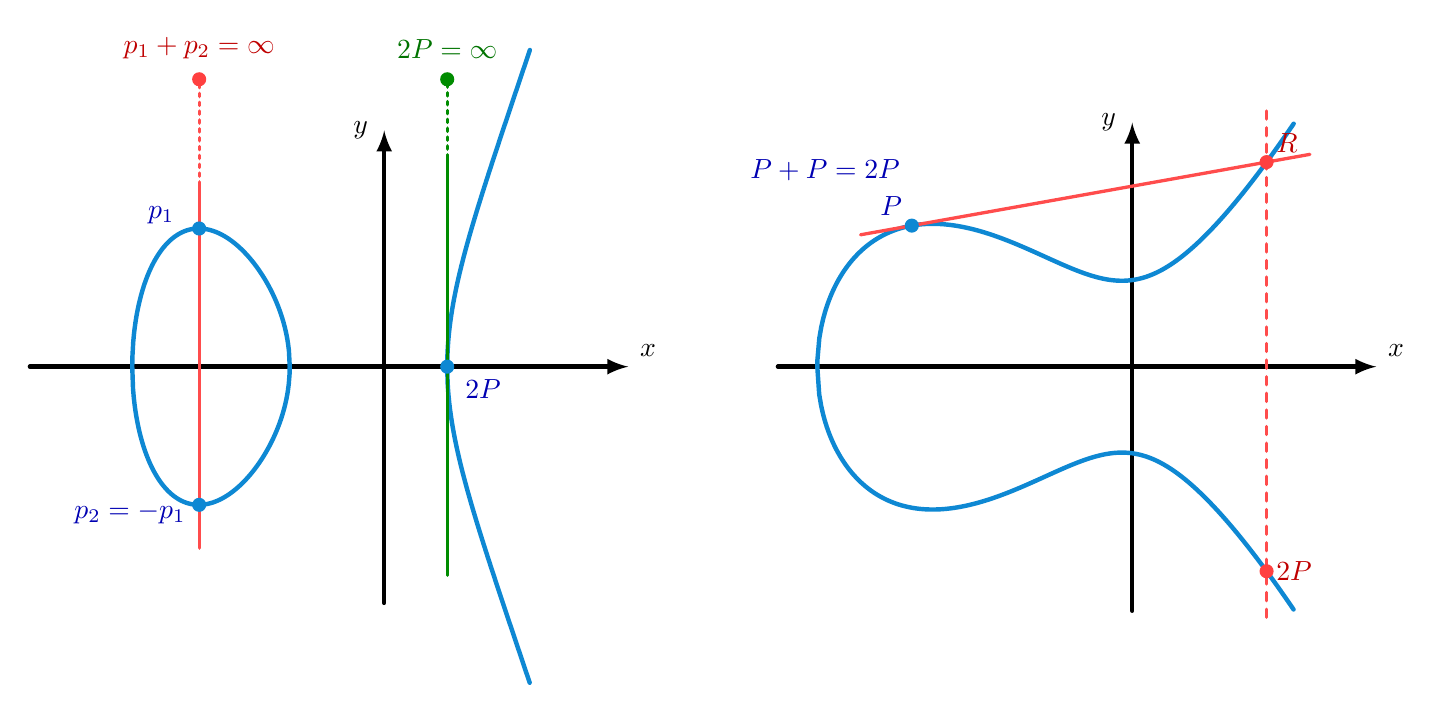
\begin{tikzpicture}[>=latex, line cap=round, line join=round]

% --- Global TikZ Styles ---
\tikzset{
    axis/.style={
        ->,
        >=latex,
        ultra thick,
        draw=black
    },
    axisline/.style={
        ultra thick,
        draw=black
    },
    elliptic/.style={
        draw=cyan!70!blue,
        line width=1.6pt
    },
    construction/.style={
        draw=red!70,
        line width=1.2pt
    },
    constructiondashed/.style={
        draw=red!70,
        dashed,
        line width=1.1pt
    },
    greenconstruction/.style={
        draw=green!55!black,
        line width=1.2pt
    },
    redpoint/.style={
        circle,
        fill=red!75,
        inner sep=1.8pt
    },
    bluepoint/.style={
        circle,
        fill=cyan!70!blue,
        inner sep=1.8pt
    },
    greenpoint/.style={
        circle,
        fill=green!55!black,
        inner sep=1.8pt
    }
}

% =========================================================================
% --- Links: p_2 = -p_1, dus p_1 + p_2 = O ---
% =========================================================================
\begin{scope}[xshift=0cm]

    \pgfmathsetmacro{\curveShift}{-1.2}

    % --- Axes ---
    \draw[axisline] (-4.5,0) -- (2.2,0);
    \draw[axis] (2.2,0) -- (3.1,0);

    \draw[axisline] (0,-3.0) -- (0,0);
    \draw[axis] (0,0) -- (0,3.0);

    \node at (3.35,0.2) {$x$};
    \node at (-0.3,3.0) {$y$};

    % --- Elliptische kromme: y^2 = x^3 - 4x, verschoven ---
    \draw[elliptic]
        plot[domain=0:-2, samples=200]
            (\x + \curveShift, {sqrt(abs(\x*\x*\x - 4*\x))})
        --
        plot[domain=-2:0, samples=200]
            (\x + \curveShift, {-sqrt(abs(\x*\x*\x - 4*\x))})
        -- cycle;

    \draw[elliptic]
        plot[domain=3.05:2, samples=200]
            (\x + \curveShift, {sqrt(abs(\x*\x*\x - 4*\x))})
        --
        plot[domain=2:3.05, samples=200]
            (\x + \curveShift, {-sqrt(abs(\x*\x*\x - 4*\x))});

    % --- Speciaal geval 1: p_2 = -p_1 ---
    \pgfmathsetmacro{\xP}{-1.15}
    \pgfmathsetmacro{\yP}{sqrt(abs(\xP*\xP*\xP - 4*\xP))}
    \pgfmathsetmacro{\XP}{\xP + \curveShift}

    % --- Verticale lijn door p_1 en p_2, verder naar oneindig ---
    \pgfmathsetmacro{\OheightRed}{3.65}

    \draw[construction]
        (\XP,{-\yP - 0.55}) -- (\XP,{\yP + 0.55});

    \draw[construction, dotted]
        (\XP,{\yP + 0.55}) -- (\XP,\OheightRed);

    \node[redpoint] at (\XP,\OheightRed) {};
    \node[red!75!black, above, yshift=4pt] at (\XP,\OheightRed) {$p_1 + p_2 = \infty$};

    % --- Blauwe punten p_1 en p_2 ---
    \node[bluepoint] at (\XP,\yP) {};
    \node[bluepoint] at (\XP,-\yP) {};

    \node[blue!70!black, left, xshift=-4pt, yshift=2pt] at ({\XP - 0.05},{\yP + 0.1}) {$p_1$};
    \node[blue!70!black, left] at ({\XP - 0.05},{-\yP - 0.1}) {$p_2=-p_1$};

    % \node[red!75!black, align=left] at (\XP,\OheightRed)
    %     {$p_1+p_2=\mathcal O$};

    % --- Speciaal geval 2: punt met verticale raaklijn ---
    \pgfmathsetmacro{\xT}{2}
    \pgfmathsetmacro{\XT}{\xT + \curveShift}

    % --- Verticale raaklijn, verder naar oneindig ---
    \pgfmathsetmacro{\OheightGreen}{3.65}

    \draw[greenconstruction]
        (\XT,-2.65) -- (\XT,2.65);

    \draw[greenconstruction, dotted]
        (\XT,2.65) -- (\XT,\OheightGreen);

    \node[greenpoint] at (\XT,\OheightGreen) {};
    \node[green!45!black, above, yshift=4pt] at (\XT,\OheightGreen) {$2P=\infty$};

    % --- Blauw punt op de x-as waar de groene lijn de kromme raakt ---
    \node[bluepoint] at (\XT,0) {};
    \node[blue!70!black, right, xshift=3pt, yshift=-8pt] at (\XT,0) {$2P$};

\end{scope}

% =========================================================================
% --- Rechts: raaklijngeval p_1 = p_2 = P ---
% =========================================================================
\begin{scope}[xshift=9.5cm]

    % We gebruiken de linkse kromme uit je oorspronkelijke figuur:
    % y^2 = x^3 + 4x^2 + x + 4,
    % met verticale compressie 0.55.

    \pgfmathsetmacro{\k}{0.55}

    % --- Axes ---
    \draw[axisline] (-4.5,0) -- (2.2,0);
    \draw[axis] (2.2,0) -- (3.1,0);

    \draw[axisline] (0,-3.1) -- (0,0);
    \draw[axis] (0,0) -- (0,3.1);

    \node at (3.35,0.2) {$x$};
    \node at (-0.3,3.1) {$y$};

    % --- Elliptische kromme ---
    \draw[elliptic]
        plot[domain=2.05:-4, samples=250]
            (\x, {\k * sqrt(abs(\x*\x*\x + 4*\x*\x + \x + 4))})
        --
        plot[domain=-4:2.05, samples=250]
            (\x, {-\k * sqrt(abs(\x*\x*\x + 4*\x*\x + \x + 4))});

    % --- Punt P en raaklijn ---
    \pgfmathsetmacro{\xP}{-2.8}
    \pgfmathsetmacro{\fP}{\xP*\xP*\xP + 4*\xP*\xP + \xP + 4}
    \pgfmathsetmacro{\yPraw}{sqrt(\fP)}
    \pgfmathsetmacro{\yP}{\k * \yPraw}

    % Helling van de raaklijn op de niet-gecomprimeerde kromme
    \pgfmathsetmacro{\mraw}{(3*\xP*\xP + 8*\xP + 1)/(2*\yPraw)}

    % Helling in de getekende, verticaal gecomprimeerde figuur
    \pgfmathsetmacro{\mdraw}{\k * \mraw}

    % Derde snijpunt R
    \pgfmathsetmacro{\xR}{\mraw*\mraw - 4 - 2*\xP}
    \pgfmathsetmacro{\yRraw}{\mraw*(\xR-\xP) + \yPraw}
    \pgfmathsetmacro{\yR}{\k * \yRraw}

    % --- Rode raaklijn ---
    \draw[construction]
        ({\xP - 0.65},{\yP - \mdraw*0.65})
        --
        ({\xR + 0.55},{\yR + \mdraw*0.55});

    % --- Spiegelingslijn door R ---
    \draw[constructiondashed]
        (\xR,{\yR + 0.65}) -- (\xR,{-\yR - 0.65});

    % --- Punten ---
    \node[bluepoint] at (\xP,\yP) {};
    \node[redpoint] at (\xR,\yR) {};
    \node[redpoint] at (\xR,-\yR) {};

    % --- Labels ---
    \node[blue!70!black, above left] at (\xP,\yP) {$P$};

    \node[red!75!black, above right] at (\xR,\yR) {$R$};

    \node[red!75!black, right] at (\xR,-\yR) {$2P$};

    \node[blue!70!black, align=left] at (-3.9,2.5)
        {$P+P=2P$};

\end{scope}

\end{tikzpicture}